\chapter{Data Set and Experimental Set Up}

\section{Data Set}

Lorem ipsum dolor sit amet, consectetur adipiscing elit. 
Sed pellentesque lacus libero, non venenatis nibh convallis quis. Suspendisse eget nisi sapien. 
Etiam vestibulum, ex vitae dignissim dignissim, augue purus molestie tellus, quis dapibus diam augue id elit. Nulla et mauris diam. Vivamus pulvinar nisl odio. Nulla ultricies pellentesque semper. 
Cras ligula metus, cursus in mattis ut, rutrum id arcu. Integer fringilla urna tincidunt nisi accumsan, ut dictum dui ultrices. 
Curabitur viverra tempus tellus, sit amet dapibus mi ornare sit amet. Proin id ligula at velit venenatis tristique. Vestibulum at magna sagittis eros lacinia rutrum id id ipsum. 
Aenean vel odio sit amet odio feugiat vulputate. Donec egestas mattis mauris, et commodo turpis mollis sit amet. Vestibulum vulputate est massa, nec aliquam augue ullamcorper nec.

\subsection{Generating Synthetic Data}

The generation of synthetic data was the first step of this experiment, and the data generated.
The aim for this step of the process was not to gain insight from the data, but rather to determine how the general structure of the setup should be.
We decided on which columns we would need to include and because we were generating it ourselves we were able to run initial tests quickly. 
A concrete example of this is setting the trajectories in the data set to all be of the same size. This choice let us set up all trajectories with the Euclidean measure and we did not have to interpolate, or otherwise handle, trajectories of unequal length. 



We generated two data sets, one complete set and one with simulated missing values. See the APPENDIX for complete code. \autoref{fig:synthetic-datasets} shows the plot of the two synthetic data sets. Note that the sets were generated randomly, and are independent from each other. Each data set contains only 26 trajectories, and there are no more than 26 points on each trajectory


\begin{figure}
    \centering
    \begin{subfigure}{.45\textwidth}
        \centering
        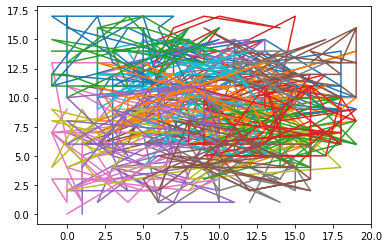
\includegraphics[width=\textwidth]{figures/SYNTHETHIC_COMPLETE.png}
        \caption{Complete data}
        \label{sfig:synthetic-comp}
    \end{subfigure}
    \hfill
    \begin{subfigure}{.45\textwidth}
        \centering
        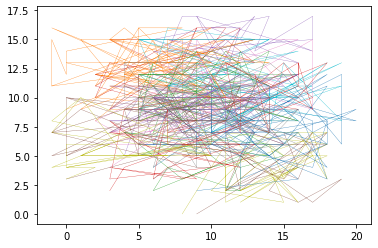
\includegraphics[width=\textwidth]{figures/SYNTHETHIC_MISSING.png}
        \caption{With simulated missing data}
        \label{sfig:synthetic-missing}
    \end{subfigure}
    \caption{Synthetic data sets of randomly generated trajectories.}
    \label{fig:synthetic-datasets}
\end{figure}

\subsection{Processing Real Data}


The real data set we chose is a taxi trajectory set (LINK). 
The data in this set contains just over 1.7 million entries, which is significantly more data than we needed for this setup.
As a part of data-preprocessing we created subsets consisting of around 500 and 100 entries. 
We deemed it unlikely that our experiments would require bigger data sets as our research goals are not geared towards efficient algorithms for huge data volumes. \autoref{fig:real-datasets} gives us a graphical representation of the data, as well as noting how many trajectories are in each set. Observe that we are unable to look at each of the several trajectories in a plot like this.  

\begin{figure}
    \centering
    \begin{subfigure}{.30\textwidth}
        \centering
        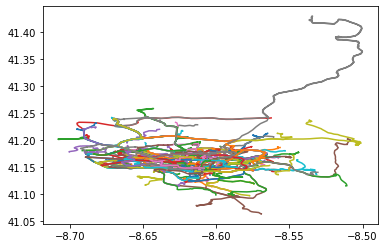
\includegraphics[width=\textwidth]{figures/REAL_MED.png}
        \caption{Subset with 551 entries}
        \label{sfig:real-med}
    \end{subfigure}
    \hfill
    \begin{subfigure}{.30\textwidth}
        \centering
        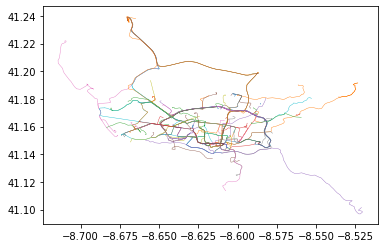
\includegraphics[width=\textwidth]{figures/REAL_MINI.png}
        \caption{Subset with 86 entries}
        \label{sfig:real-mini}
    \end{subfigure}
    \hfill
    \begin{subfigure}{.30\textwidth}
        \centering
        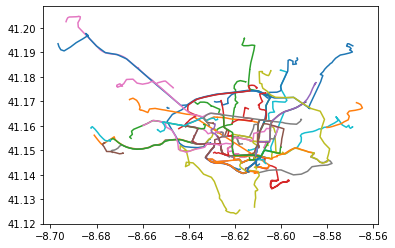
\includegraphics[width=\textwidth]{figures/REAL_NO_MISS.png}
        \caption{Subset with 61 entries and no missing data}
        \label{sfig:real-no-miss}
    \end{subfigure}
    \caption{Synthetic data sets of randomly generated trajectories.}
    \label{fig:real-datasets}
\end{figure}


\section{Technical environment}
The experiments carried out in this thesis were executed in Jupyter Notebooks[REF] which were hosted by Google in Google Colab[REF].

The motivation for picking this environment is two fold: Firstly, we appreciated the ability to work “from anywhere” and by using a cloud-based service such as Google Colab, we were able to achieve this. 
Another advantage of using Google's solution is that we got a lot of free GPU power. Secondly, Jupyter Notebooks are well suited to note taking alongside coding. 

\subsection{Jupyter Notebooks}
The base components of all Jupyter Notebook are the input/output cells which themselves can be grouped together. 
Among other options, the document can contain code, markdown and TeX. In short, the transition between coding and writing was incredibly smooth which was conducive to a better workflow.


////INSERT some photo of Jupyter notebook


\subsection{Google Colab}
asa






























